\begin{frame}{Tomato leaf curl virus disease (TYLCVD)}
    \only<1>{
        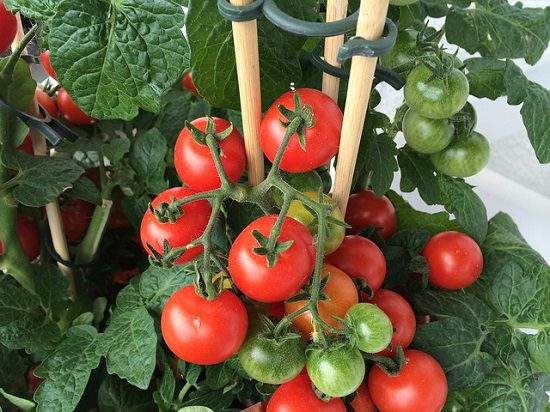
\includegraphics[width=0.7\textwidth,keepaspectratio]{assets/healty_leaf}
    }
    \only<2>{
        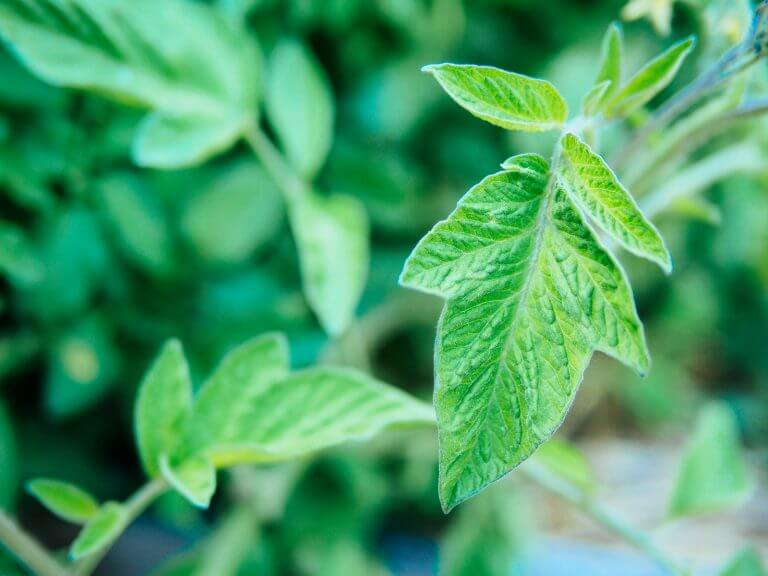
\includegraphics[width=0.7\linewidth]{assets/healty_tomato_leaf}
    }
\end{frame}
%%%%%%%%%%%%%%%%%%%%%%%%%%%%%%%%%%%%%%%%%%%%%%%%%%%%%%%%
\begin{frame}{Tomato leaf curl virus disease (TYLCVD)}
    \begin{textblock*}{65mm}(73mm, 10mm)
        \only<1->{
            \includegraphics[scale=0.08,%
                keepaspectratio]{assets/TYLCV_leaflet_cropped}
        }
    \end{textblock*}
    \begin{textblock*}{60mm}(5mm, 10mm)
        \begin{greenbox}{}
            \begin{itemize}[<+->]
                \item
                    Tomato plants \hl{infected early}
                    are severely stunted and will
                    \hl{not produce fruit}
                \item
                    Leaflets are small and yellowed 
                    with edges that curl upwards
                \item
                    Flowers either do not develop or 
                    fall off
                \item
                    When \hl{older plants} are 
                    infected, fruit that is already
                    forming ripens normally, but 
                    \hl{no new fruit} 
                    is formed after the infection
                \item
                    TYLCV can be confused with several 
                    other conditions such as tomato big 
                    bud, herbicide damage and phosphate 
                    or magnesium deficiency
            \end{itemize}
        \end{greenbox}
    \end{textblock*}
 \end{frame}
%%%%%%%%%%%%%%%%%%%%%%%%%%%%%%%%%%%%%%%%%%%%%%%%%%%%%%%%
\begin{frame}{Tomato leaf curl virus disease (TYLCVD)}
    \begin{textblock*}{60mm}(67mm, 30mm)
        \only<1-4>{
        \includegraphics[width=\linewidth]{assets/Silverleaf_whitfly_large_rotated}
        }
        \only<5-6>{
        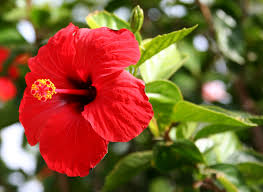
\includegraphics[width=\linewidth]{assets/ibicum_rosanensis}    
    }
    \end{textblock*}
    \begin{textblock*}{55mm}(10mm, 10mm)
        \begin{greenbox}{Spread}
            \begin{itemize}[<+->]
                \item
                    \hl{TYLCV} is spread by the insect 
                    silverleaf whitefly (Bemisia tabaci 
                    B biotype)
                \item
                    Silverleaf whiteflies pick up the 
                    virus by feeding on infected host 
                    plants. The whiteflies then 
                    spread the virus to healthy plants 
                    \hl{ which show the symptoms 
                    10 to 21 days later}
                \item
                    Silverleaf whiteflies are 
                    \hl{common} in many countries and 
                    \hl{feed} on \hl{many} types of 
                    \hl{plants}
                \item
                    More than 22 species,
                    including both annuals and perennials, are also
                    known hosts of TLCV.
            \end{itemize}
        \end{greenbox}
    \end{textblock*}
\end{frame}
%%%%%%%%%%%%%%%%%%%%%%%%%%%%%%%%%%%%%%%%%%%%%%%%%%%%%%%%
%%%%%%%%%%%%%%%%%%%%%%%%%%%%%%%%%%%%%%%%%%%%%%%%%%%%%%%%
\begin{frame}{}
    \begin{textblock*}{55mm}(5mm, 2mm)
        \begin{bluebox}{Control}
            Cultural Control
            \begin{itemize}[<+->]
                \item
                    Physical barriers
                \item
                    Planting dates
                \item
                    \textbf{Replanting of infected plants}
                \item
                    Host plant resistance
            \end{itemize}
            Biological Control
            \tcblower
            \begin{itemize}[<+->]
                \item
                    Parasitoids
                \item
                    Predators
                \item
                    Fungi
            \end{itemize}
        \end{bluebox}
    \end{textblock*}
%%%%%%%%%%    
    \begin{textblock*}{55mm}(5mm, 62mm)
        \only<5>{
            \begin{center}
                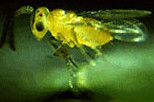
\includegraphics[width=.7\linewidth]{assets/Eretmocerus} 
            \end{center}
        }
        \only<6>{
            \begin{center}
            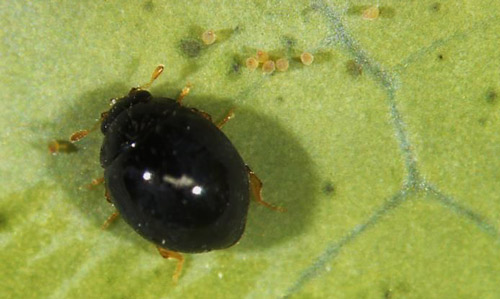
\includegraphics[width=.7\linewidth]{assets/Delphastus_catalinae01} 
            \end{center}
        }
        \only<7>{
            \begin{center}
                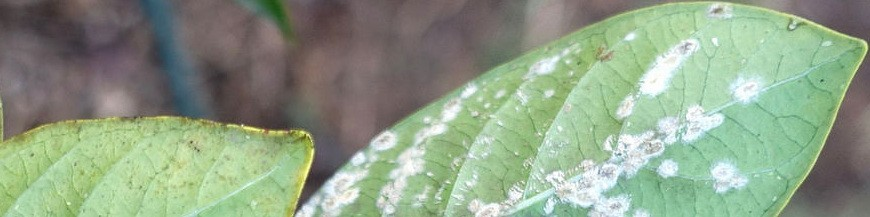
\includegraphics[width=\linewidth]{assets/verticillium-lecani}
            \end{center}
        }
    \end{textblock*}
%
    \begin{textblock*}{60mm}(65mm, 2mm)
        \begin{yellowbox}{Insecticides}
            \begin{itemize}
                \item 
                    pymetrozine
                 \item 
                    zeta-cypermethrin / bifenthrin
            \end{itemize}
        \end{yellowbox}
        \begin{graybox}{}
            \begin{bibunit}[apalike]
                \nocite{Shun-xiang2001}
                \nocite{Smith2014}
                \putbib
            \end{bibunit}
        \end{graybox}
    \end{textblock*}
\end{frame}
